
\documentclass{article}
\usepackage[spanish]{babel}
\usepackage[utf8]{inputenc}
\usepackage{amssymb, amsmath, amsbsy, wasysym}
\usepackage{multirow}
\usepackage{graphicx}
\usepackage{hyperref}
\title{Práctica 6\\Redes de computadoras}
\author{Emmanuel Peto Gutiérrez}
\begin{document}
\maketitle

\section{Pasos para desarrollar la práctica}

Tomando la red de la práctica 5, se agregan otras dos subredes: una de Google y otra de Telmex.

Para la de Google se agregan los siguientes dispositivos.

\begin{center}
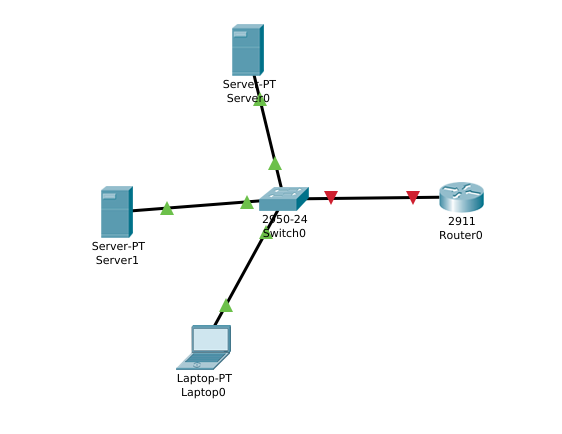
\includegraphics[scale=0.3]{imagenes/1}
\end{center}

Para la de Telmex los sigiuentes dispositivos.

\begin{center}
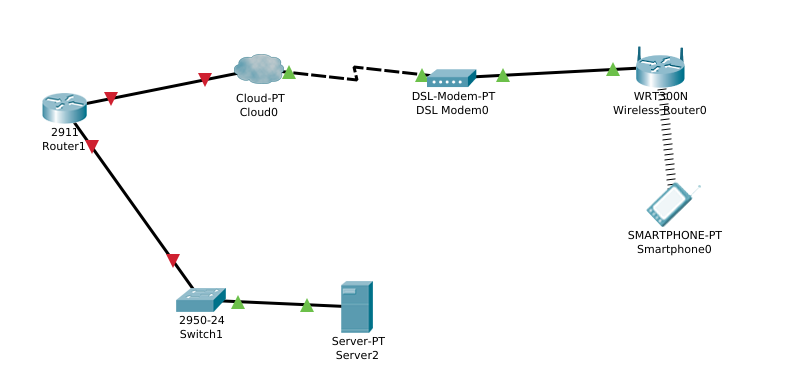
\includegraphics[scale=0.3]{imagenes/2}
\end{center}

Se configuran las redes de Google y Telmex con los siguientes parámetros.

\begin{center}
\begin{tabular}{|c|c|c|c|c|}
\hline
\textbf{Nombre} & \textbf{IP} & \textbf{Máscara} & \textbf{Gateway} & \textbf{DNS} \\ \hline
ns.google.com.mx & 216.58.193.2 & 255.255.255.0 & 216.58.193.1 & NA \\ \hline
www.google.com.mx & 216.58.193.3 & 255.255.255.0 & 216.58.193.1 & 216.58.193.2 \\ \hline
Laptop1 & 216.58.193.10 & 255.255.255.0 & 216.58.193.1 & 216.58.193.2 \\ \hline
\end{tabular}
\end{center}

\begin{center}
\begin{tabular}{|c|c|c|c|c|}
\hline
\textbf{Nombre} & \textbf{IP} & \textbf{Máscara} & \textbf{Gateway} & \textbf{DNS} \\ \hline
ns.telmex.com.mx & 201.124.197.10 & 255.255.255.0 & 201.124.197.1 & NA \\ \hline
\end{tabular}
\end{center}

\begin{center}
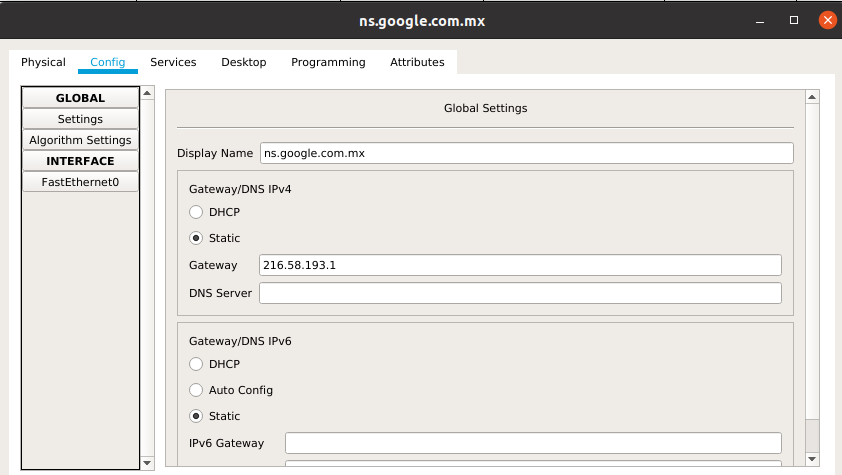
\includegraphics[scale=0.3]{imagenes/3}

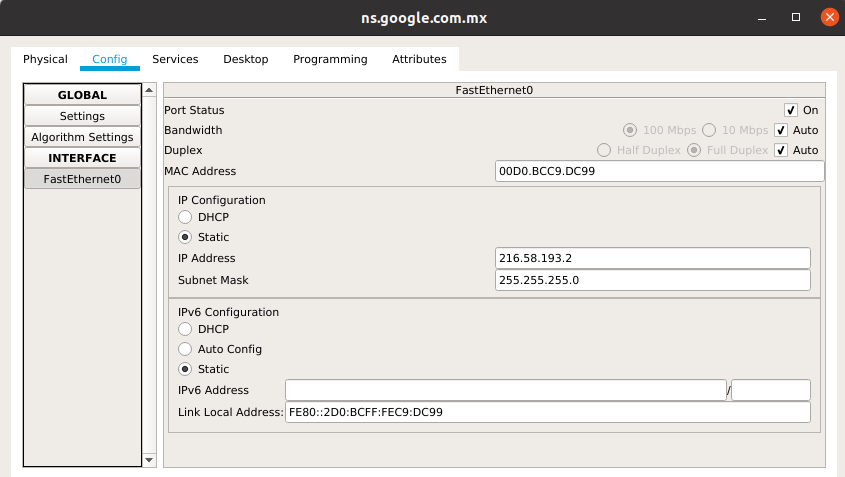
\includegraphics[scale=0.3]{imagenes/4}

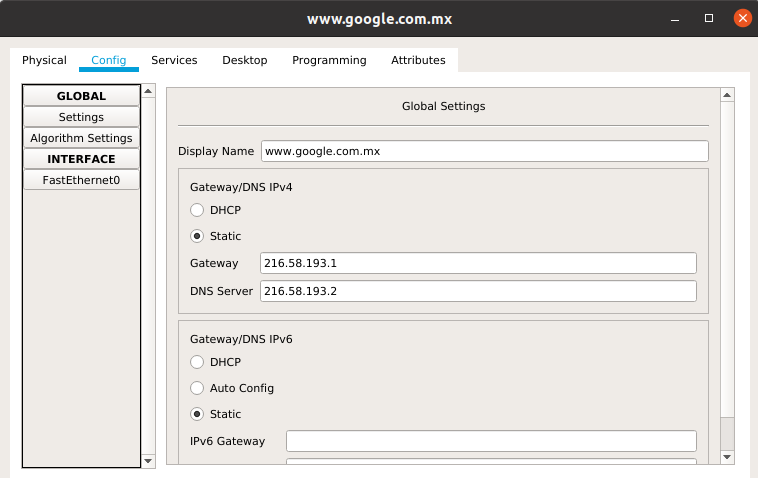
\includegraphics[scale=0.3]{imagenes/5}

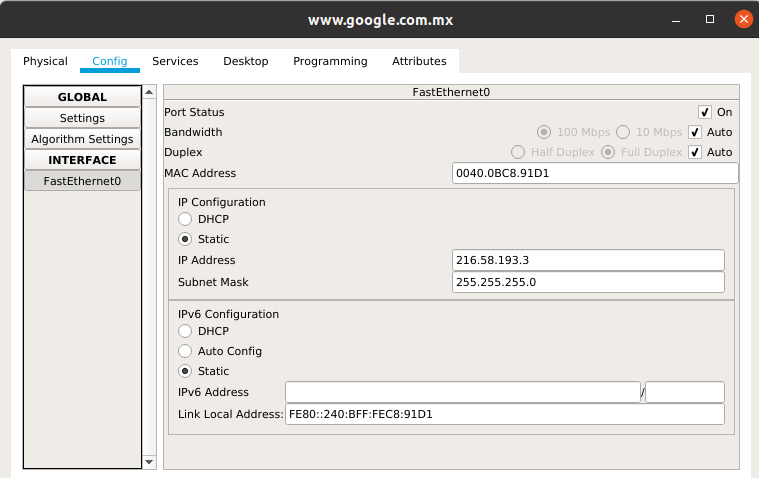
\includegraphics[scale=0.3]{imagenes/6}

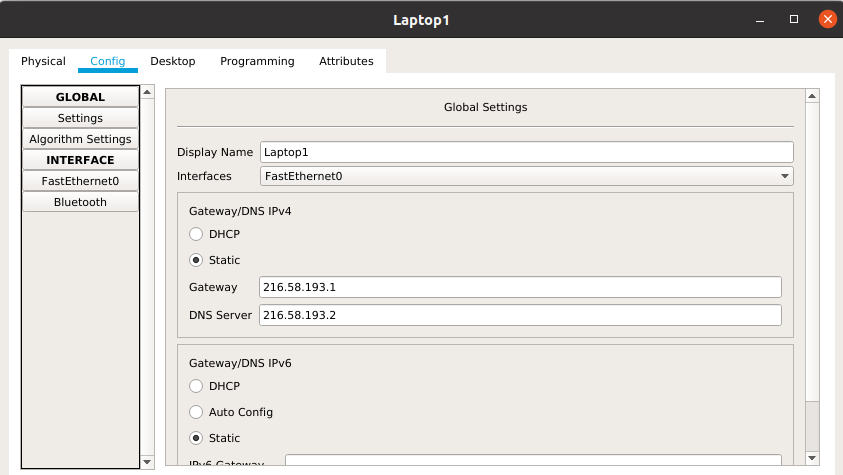
\includegraphics[scale=0.3]{imagenes/7}

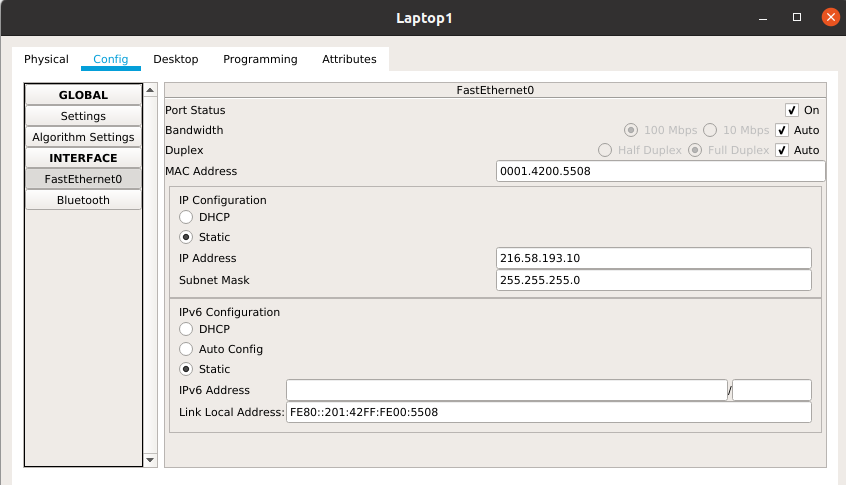
\includegraphics[scale=0.3]{imagenes/8}

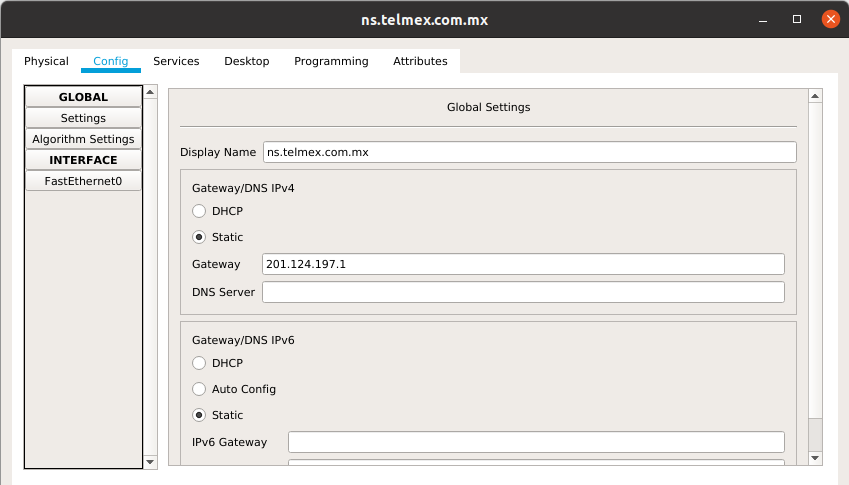
\includegraphics[scale=0.3]{imagenes/9}

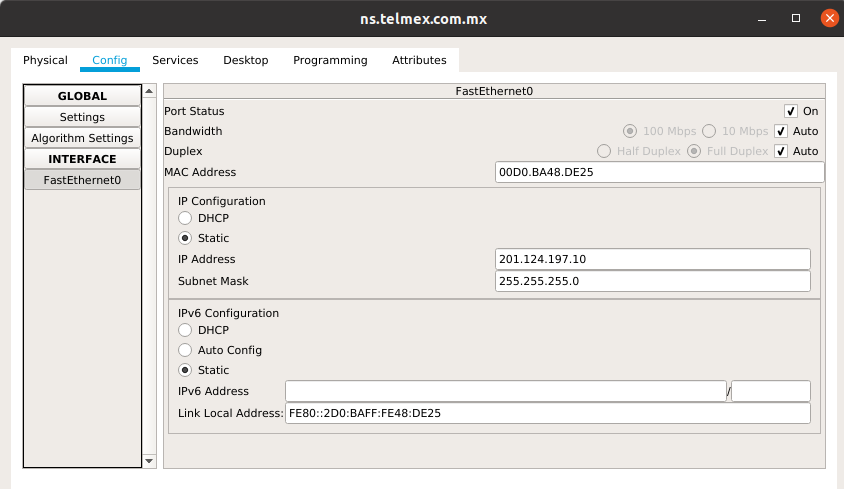
\includegraphics[scale=0.3]{imagenes/10}
\end{center}

Se configura el Wireless Router del hogar en la subred de Telmex.

\begin{center}
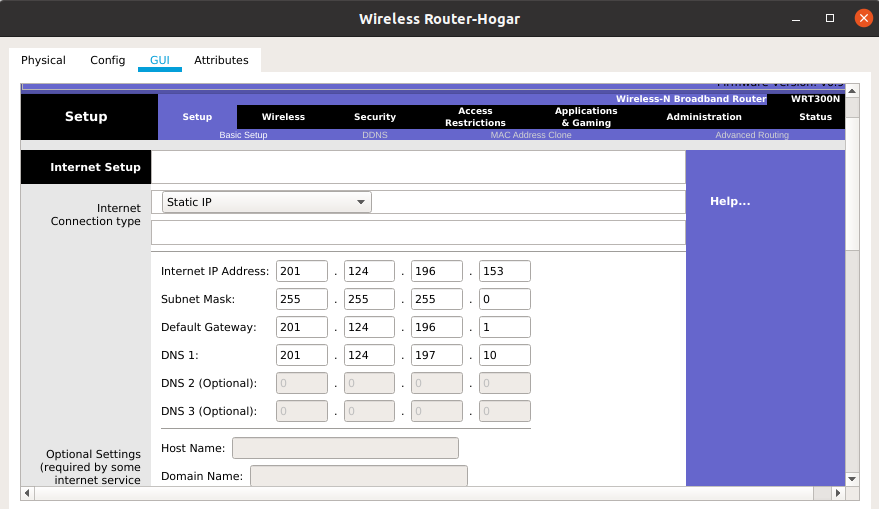
\includegraphics[scale=0.3]{imagenes/11}

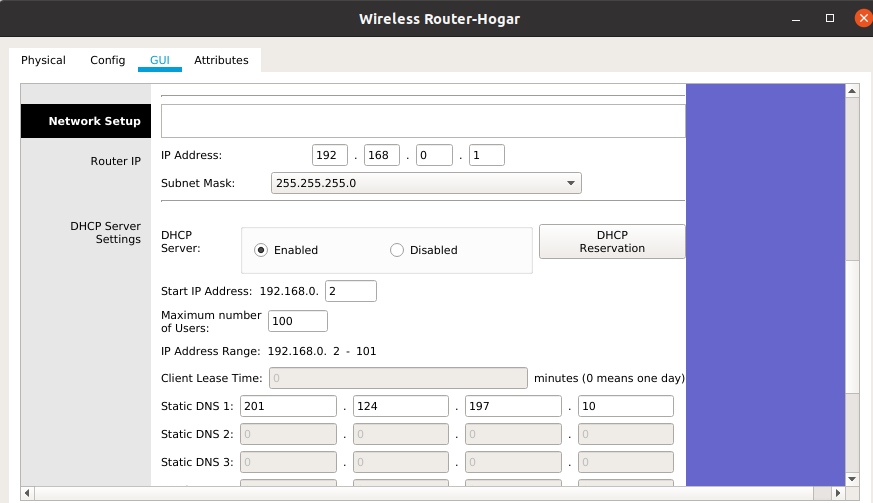
\includegraphics[scale=0.3]{imagenes/12}

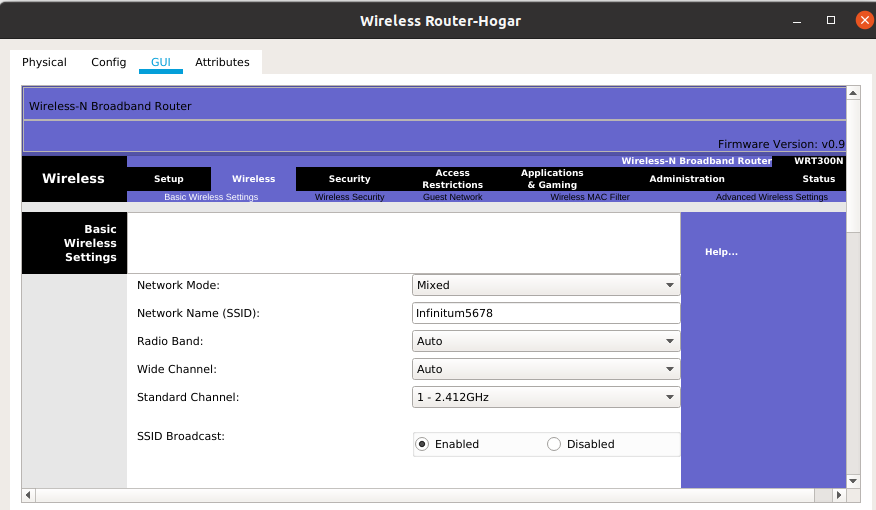
\includegraphics[scale=0.3]{imagenes/13}
\end{center}

Se conecta el Smartphone al router.

\begin{center}
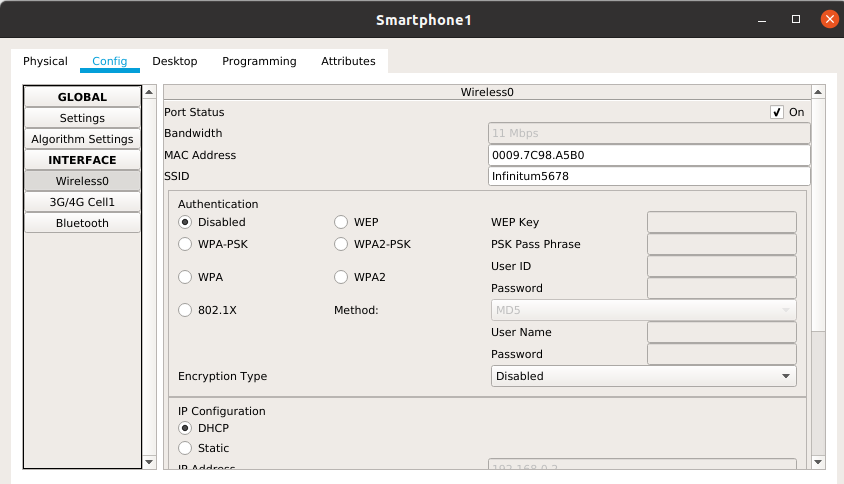
\includegraphics[scale=0.3]{imagenes/14}
\end{center}

Se configura el dispositivo Cloud-PT con el nombre de Red Infinitum.

\begin{center}
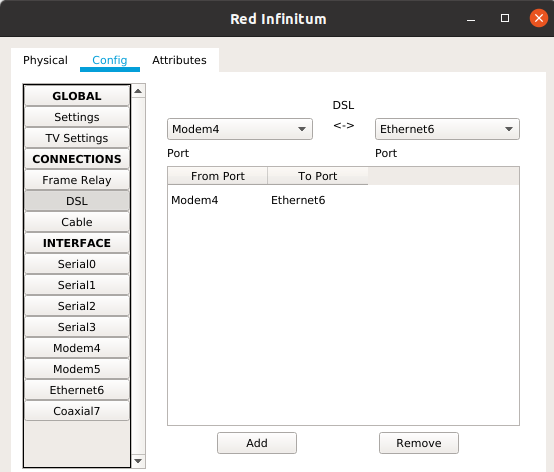
\includegraphics[scale=0.3]{imagenes/15}
\end{center}

Después, se configura el sitio web de Google, como se hizo con los sitios en la práctica anterior.

\begin{center}
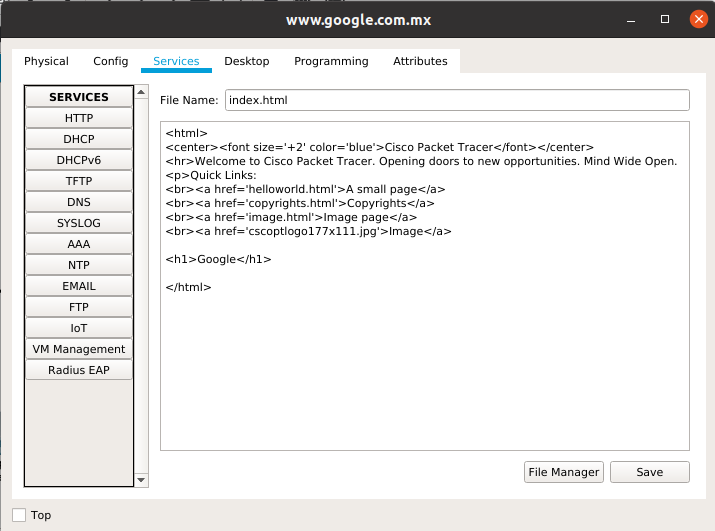
\includegraphics[scale=0.3]{imagenes/16}
\end{center}

Se deben configurar los servidores DNS que se acaban de agregar, además de agregar registros a los servidores de Ciencias y DGTIC.

\begin{center}
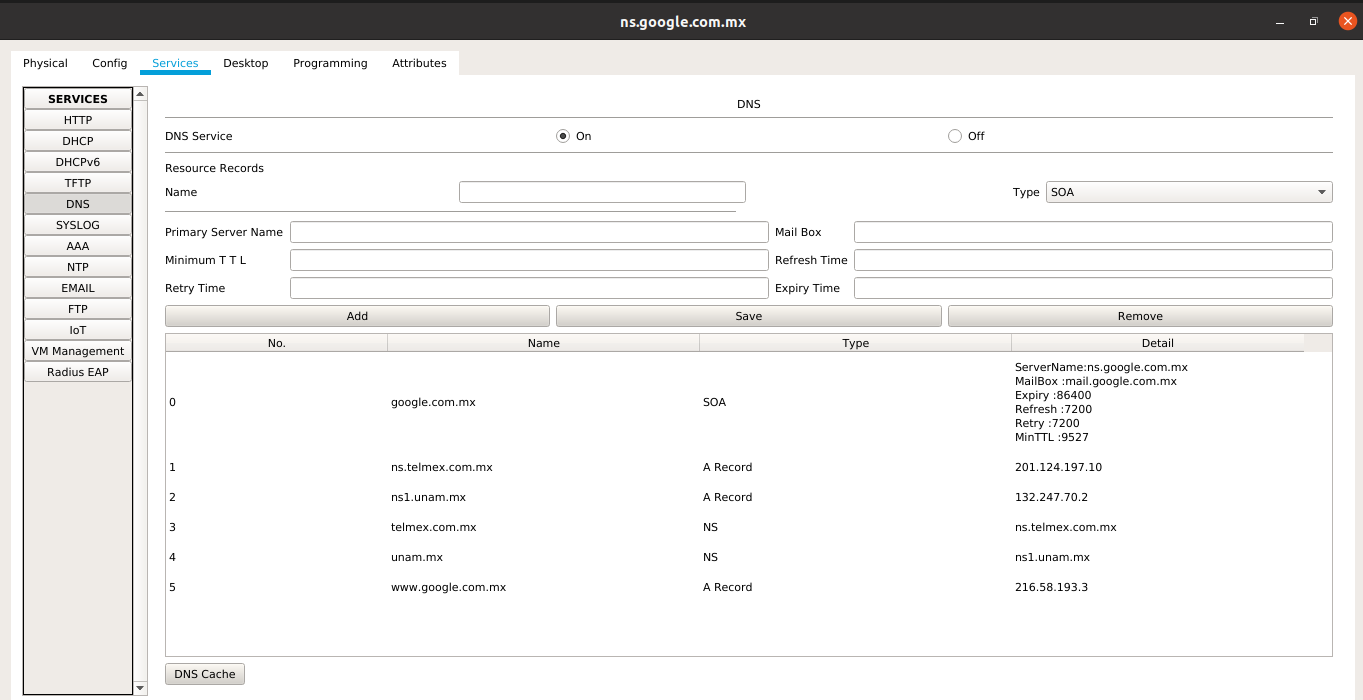
\includegraphics[scale=0.3]{imagenes/17}

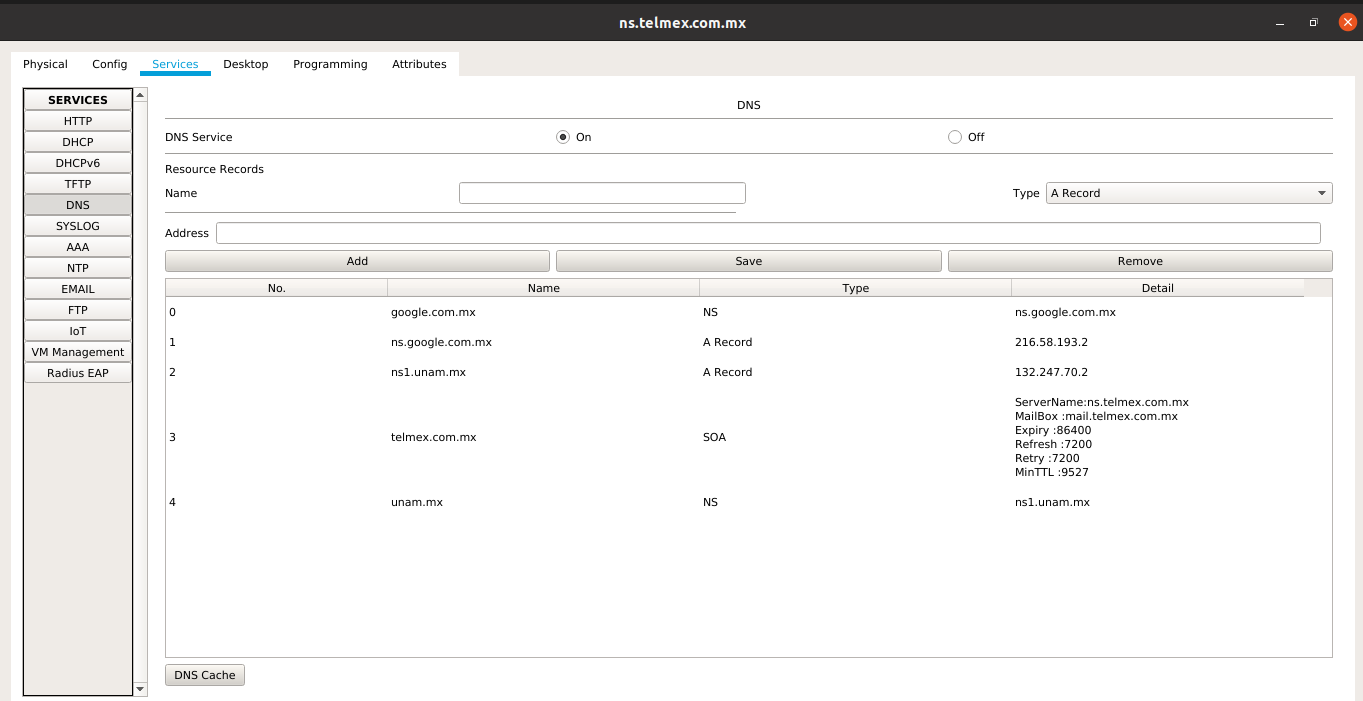
\includegraphics[scale=0.3]{imagenes/18}

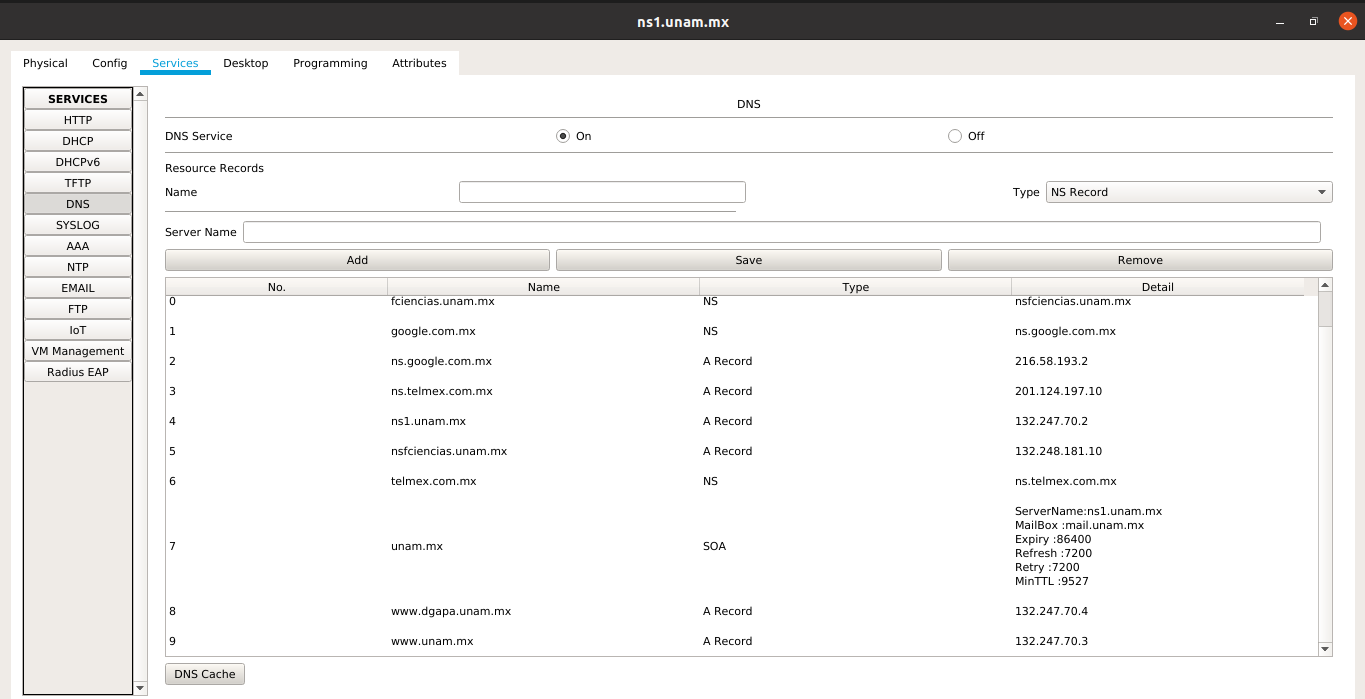
\includegraphics[scale=0.3]{imagenes/19}

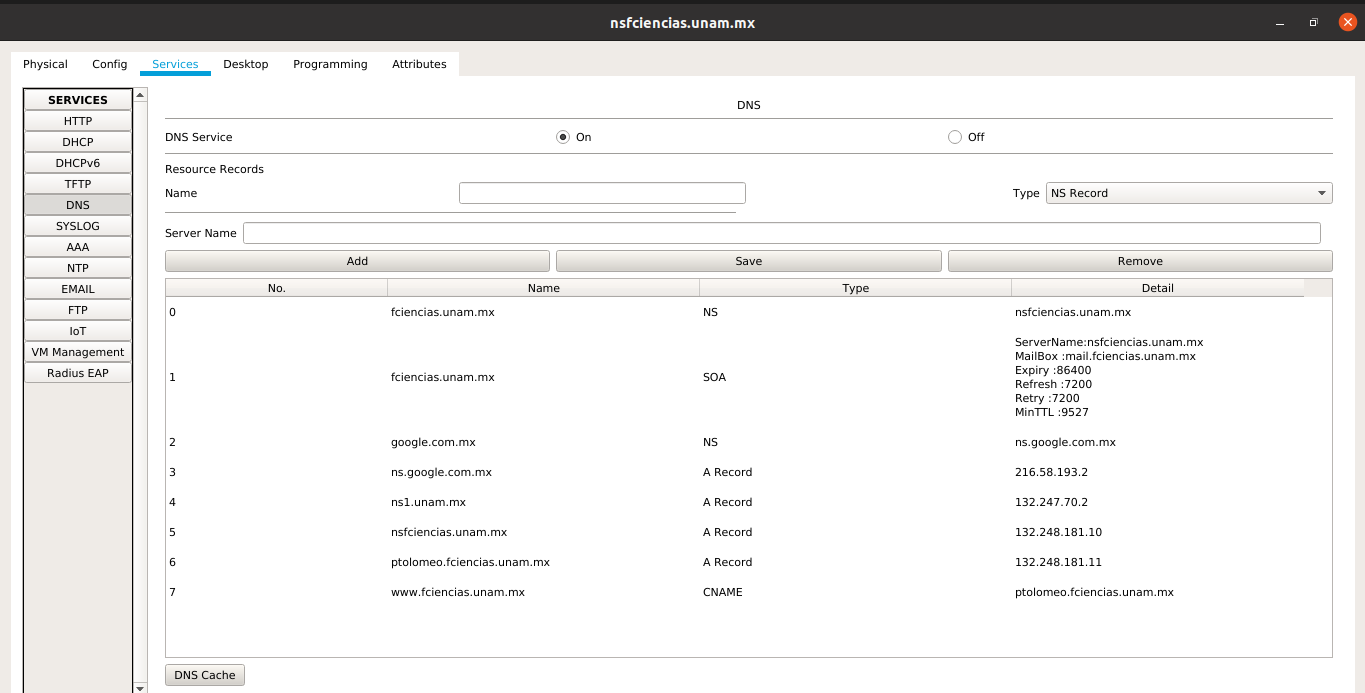
\includegraphics[scale=0.3]{imagenes/20}
\end{center}

Se cambian los \textit{display name} y \textit{hostname} de los routers de Google, UNAM y Telmex.

\begin{center}
\begin{tabular}{|c|c|}
\hline
\textbf{Dispositivo} & \textbf{Nombre} \\ \hline
Router UNAM & R-UNAM \\ \hline
Router Google & R-Google \\ \hline
Router Telmex & R-Telmex \\ \hline
\end{tabular}
\end{center}

Para cada uno de los tres routers se agrega la interfaz HWIC-2T.

\begin{center}
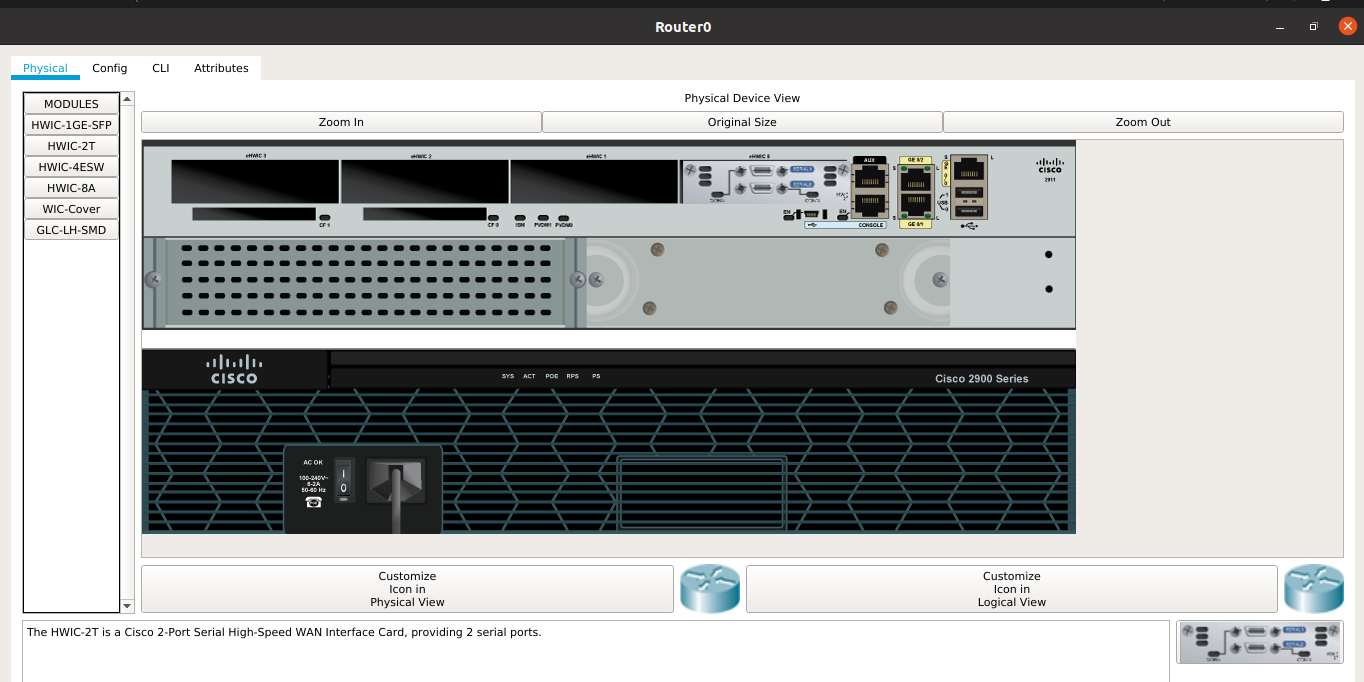
\includegraphics[scale=0.3]{imagenes/21}
\end{center}

Se configuran los routers y el SW-Core como en la práctica anterior, además se ponen configuraciones para poder agregar los cables DTE o DCE. En este paso se coloca la dirección de cada cable.

\begin{center}
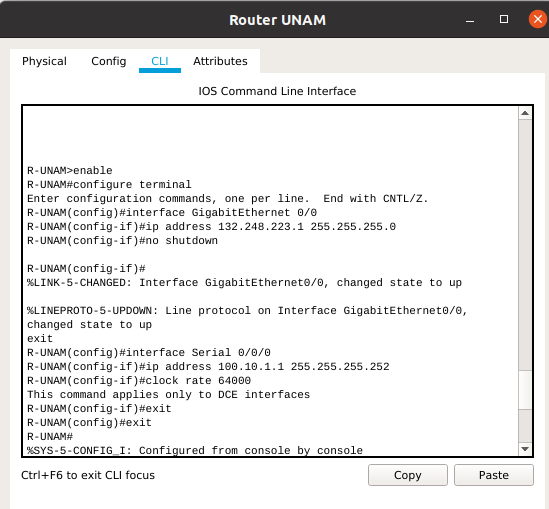
\includegraphics[scale=0.3]{imagenes/22}

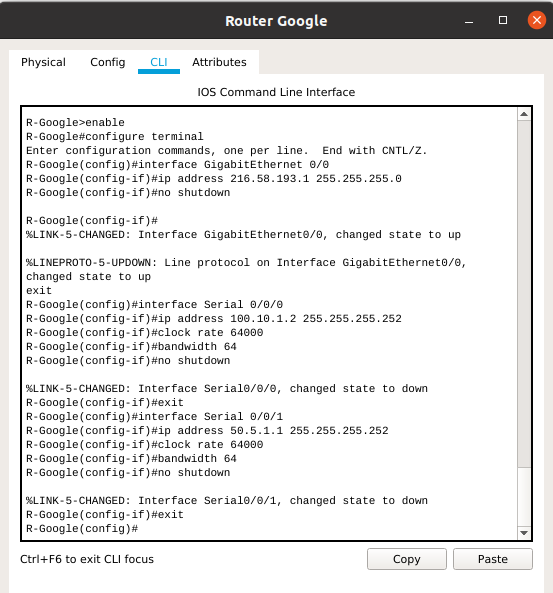
\includegraphics[scale=0.3]{imagenes/23}

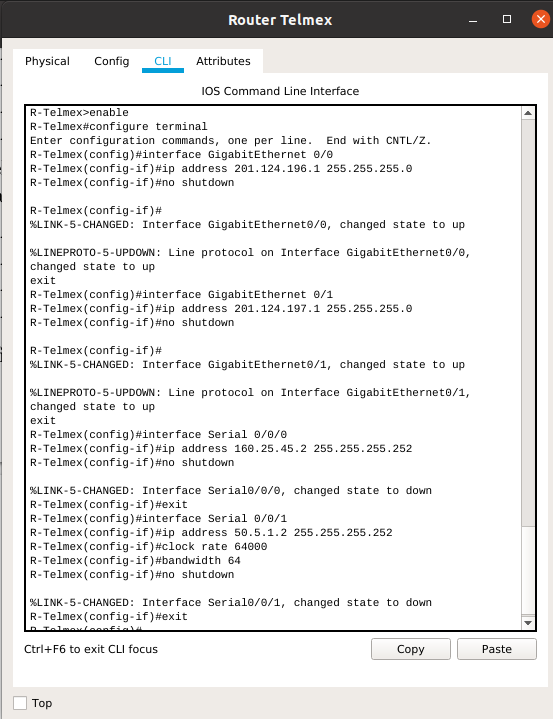
\includegraphics[scale=0.3]{imagenes/24}

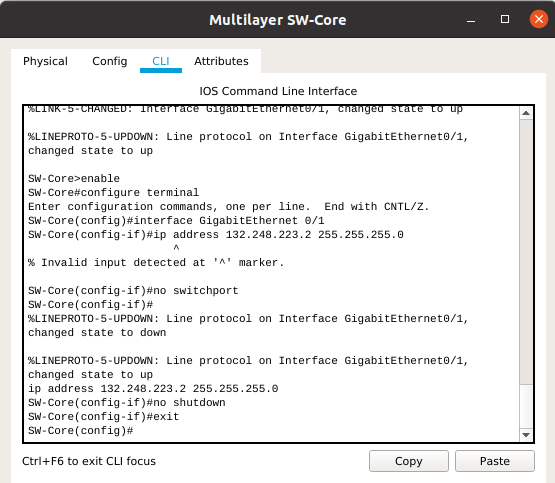
\includegraphics[scale=0.3]{imagenes/25}
\end{center}

Hay que configurar las rutas dinámicas en todos los routers y el SW-Core. Para eso se usa RIP 2.

\begin{center}
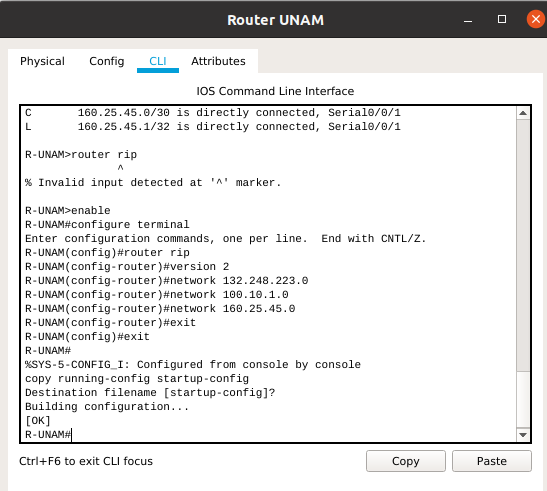
\includegraphics[scale=0.3]{imagenes/26}

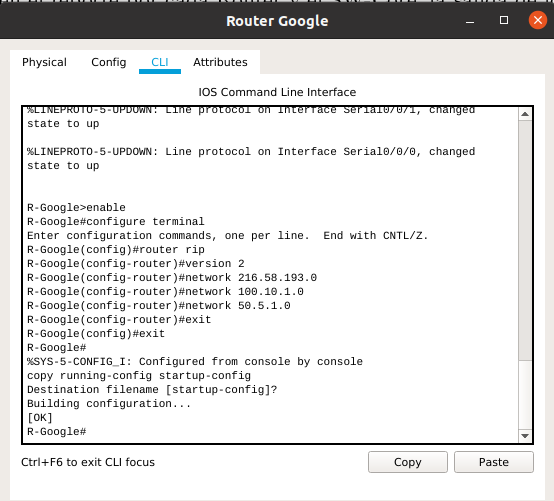
\includegraphics[scale=0.3]{imagenes/27}

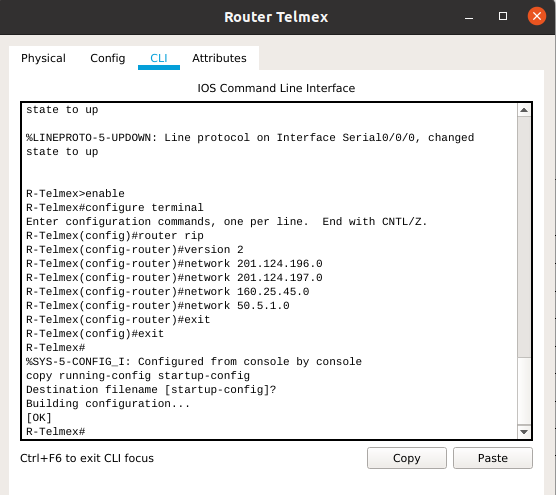
\includegraphics[scale=0.3]{imagenes/28}

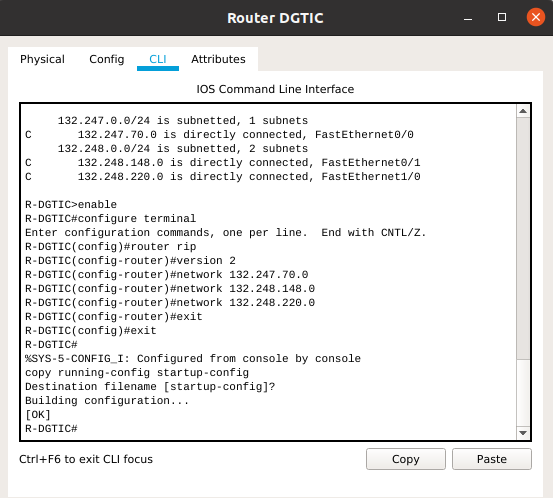
\includegraphics[scale=0.3]{imagenes/29}

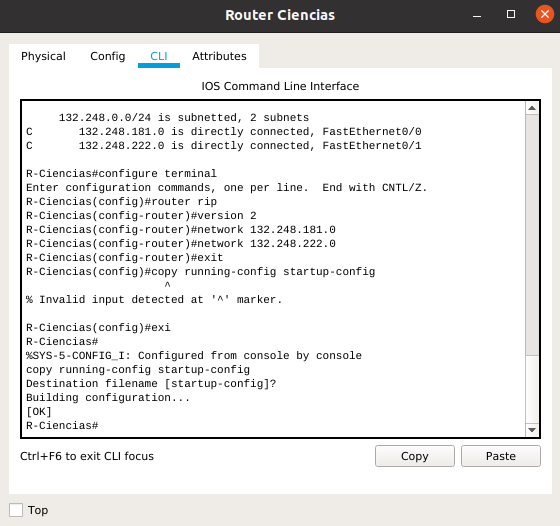
\includegraphics[scale=0.3]{imagenes/30}

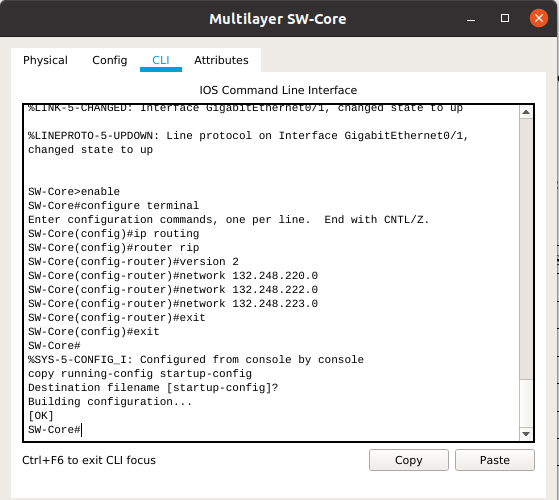
\includegraphics[scale=0.3]{imagenes/39}

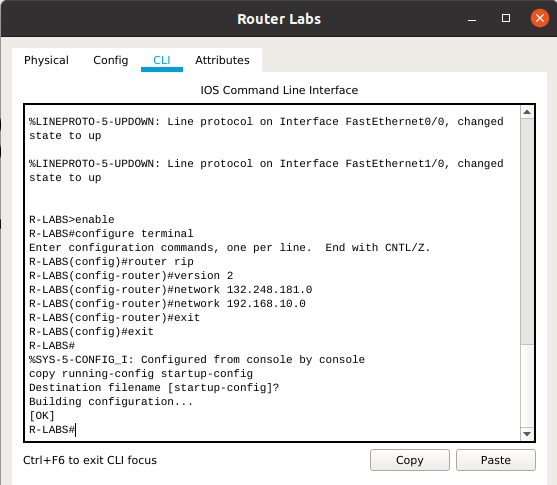
\includegraphics[scale=0.3]{imagenes/44}
\end{center}

Se puede ver la configuración con los comandos: \texttt{show ip route} y \texttt{show ip interface brief}.

\begin{center}
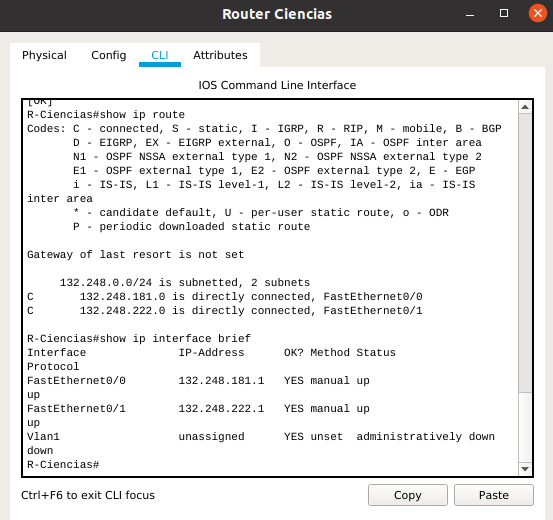
\includegraphics[scale=0.3]{imagenes/31}

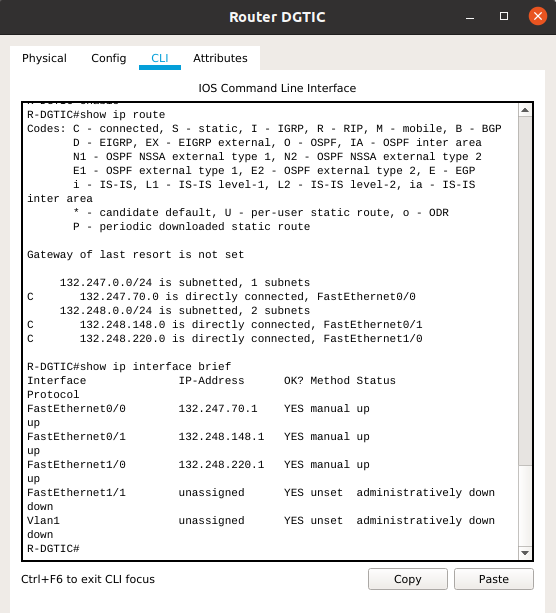
\includegraphics[scale=0.3]{imagenes/32}

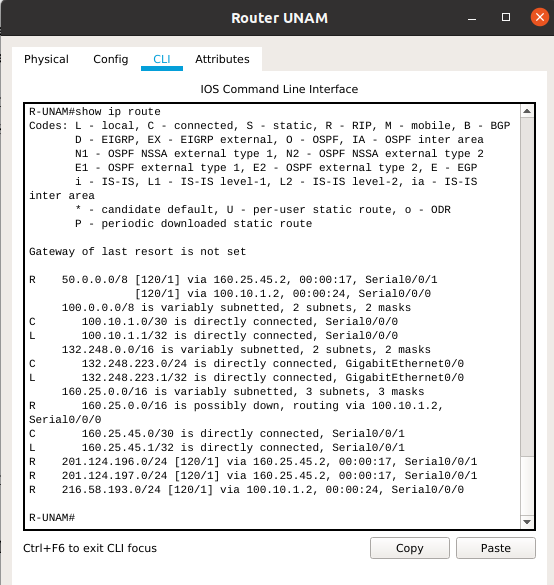
\includegraphics[scale=0.3]{imagenes/33}

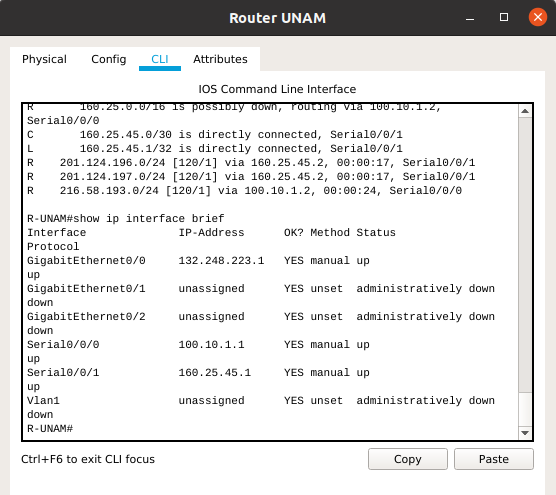
\includegraphics[scale=0.3]{imagenes/34}

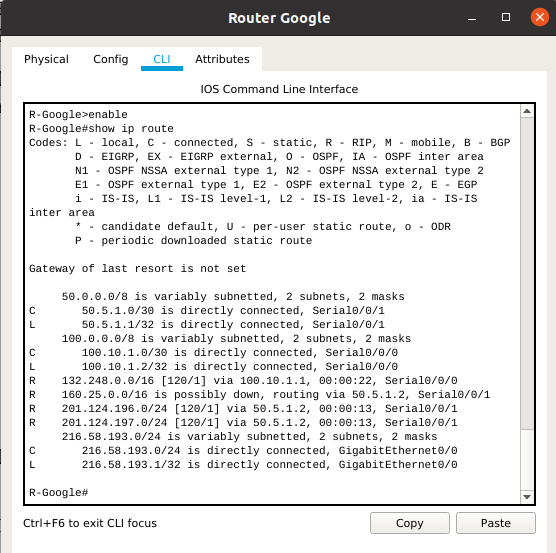
\includegraphics[scale=0.3]{imagenes/35}

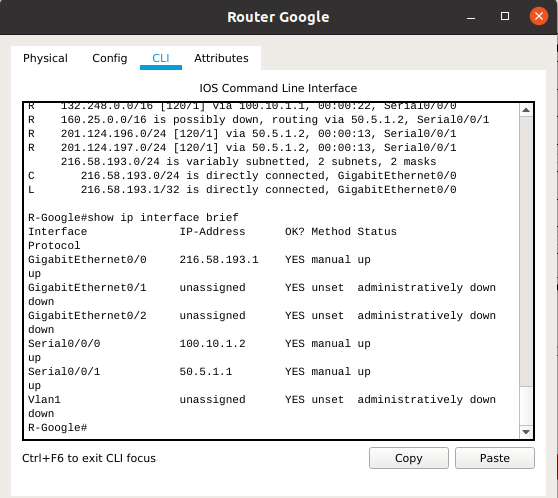
\includegraphics[scale=0.3]{imagenes/36}

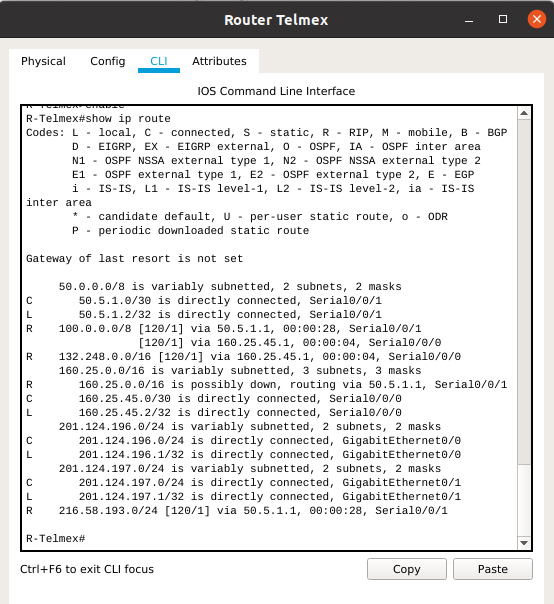
\includegraphics[scale=0.3]{imagenes/37}

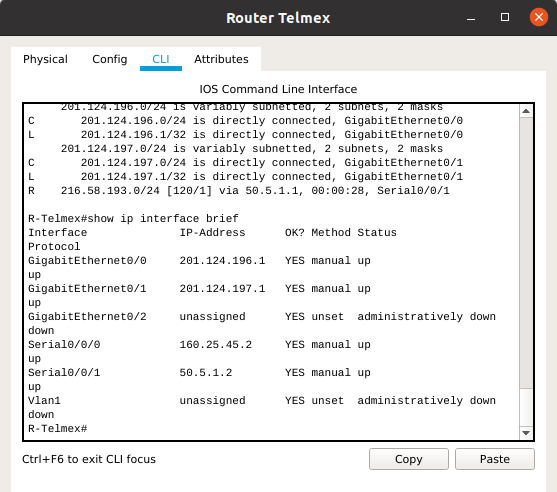
\includegraphics[scale=0.3]{imagenes/38}

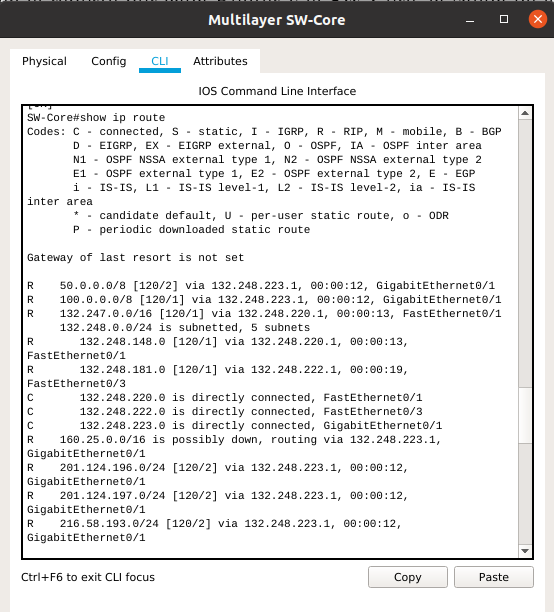
\includegraphics[scale=0.3]{imagenes/40}

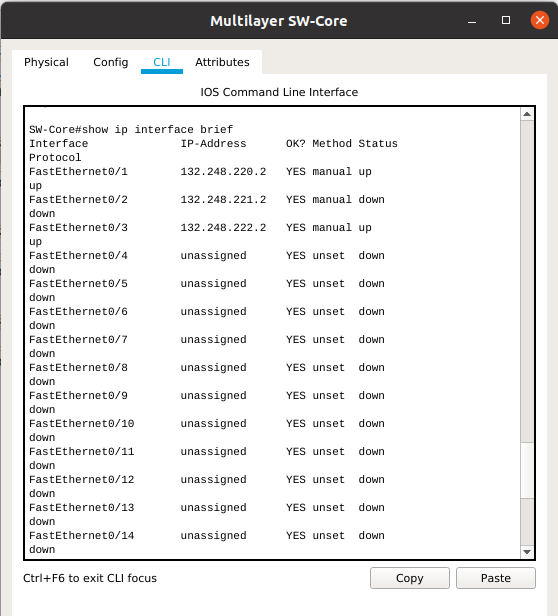
\includegraphics[scale=0.3]{imagenes/41}

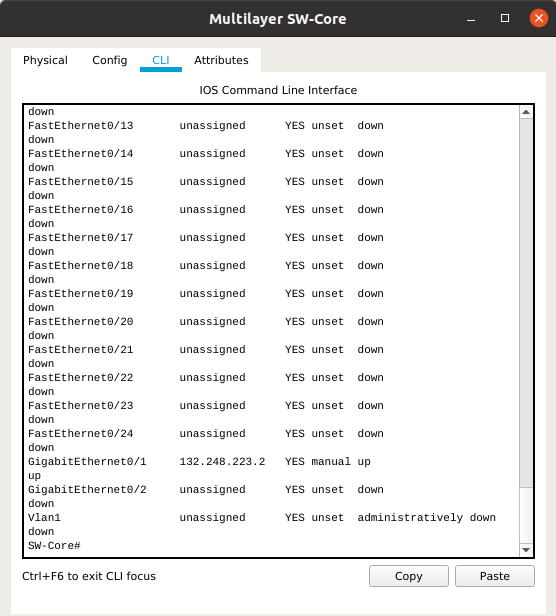
\includegraphics[scale=0.3]{imagenes/42}

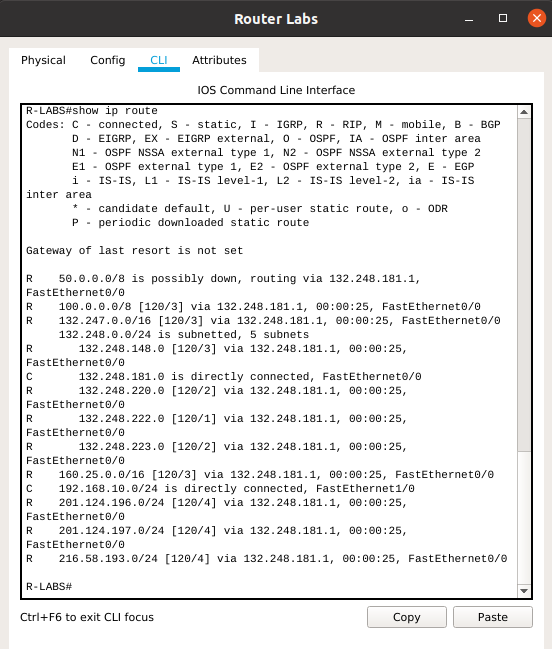
\includegraphics[scale=0.3]{imagenes/45}

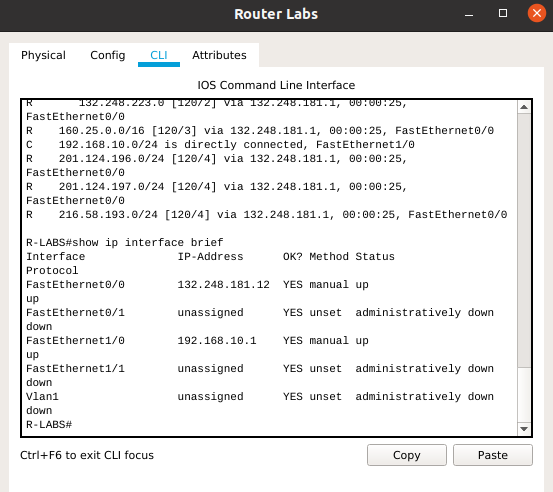
\includegraphics[scale=0.3]{imagenes/46}
\end{center}

Finalmente hay que comprobar que se puede acceder a los servidores web desde otras subredes.

\begin{center}
\begin{tabular}{|c|c|}
\hline
\textbf{Dispositivo} & \textbf{Sitio web} \\ \hline
PC1-DGTIC & www.google.com.mx \\ \hline
A-PC2 & www.google.com.mx \\ \hline
\multirow{2}{*}{Laptop1} & www.unam.mx \\
& www.fciencias.unam.mx\\ \hline
\multirow{3}{*}{Smartphone2} & www.google.com.mx \\
& www.unam.mx \\
& www.fciencias.unam.mx \\ \hline
\end{tabular}
\end{center}

\begin{center}
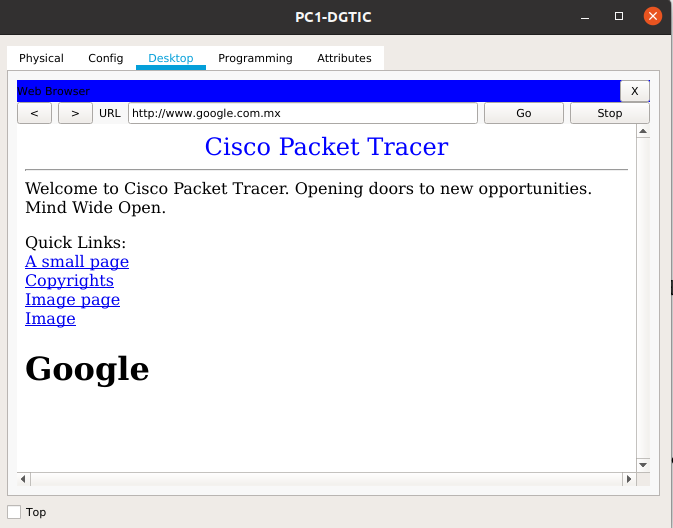
\includegraphics[scale=0.3]{imagenes/43}

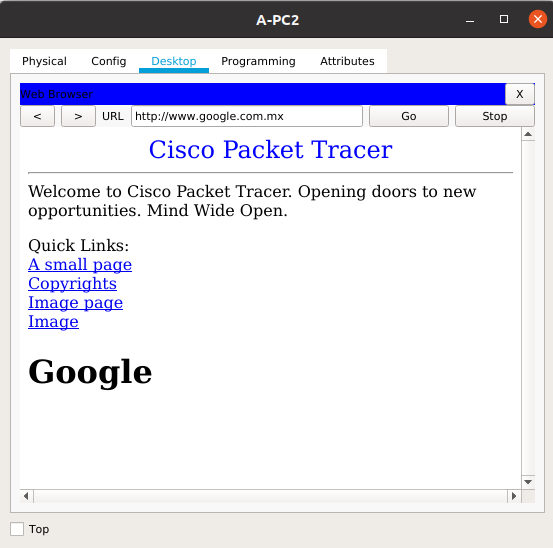
\includegraphics[scale=0.3]{imagenes/47}

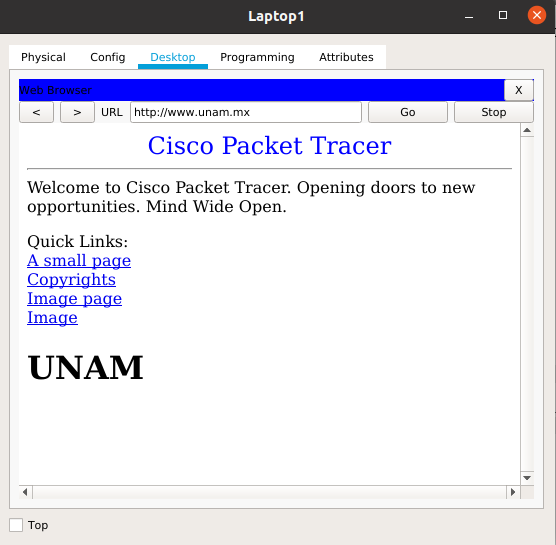
\includegraphics[scale=0.3]{imagenes/48}

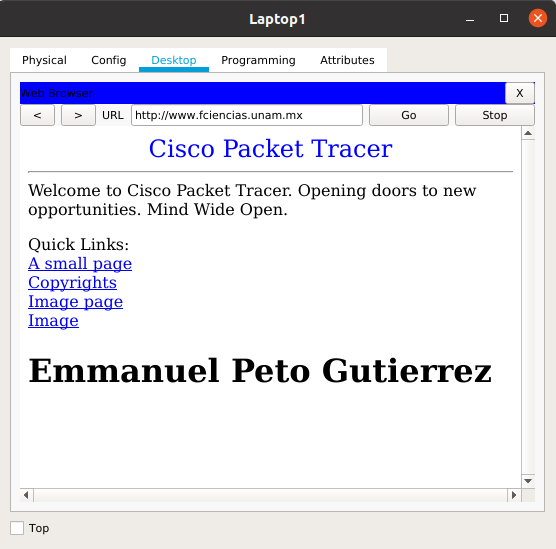
\includegraphics[scale=0.3]{imagenes/49}

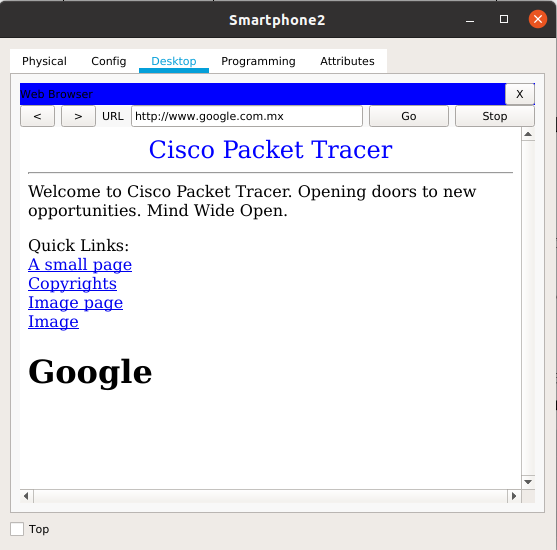
\includegraphics[scale=0.3]{imagenes/50}

\includegraphics[scale=0.3]{imagenes/51}

\includegraphics[scale=0.3]{imagenes/52}
\end{center}

Después de ingresar a dichas páginas web cambia la memoria caché de cada servidor DNS.

\begin{center}
Facultad de Ciencias

\includegraphics[scale=0.3]{imagenes/53}

UNAM

\includegraphics[scale=0.3]{imagenes/54}

Google

\includegraphics[scale=0.3]{imagenes/55}

Telmex

\includegraphics[scale=0.3]{imagenes/56}
\end{center}

La red final es la siguiente.

\begin{center}
\includegraphics[scale=0.3]{imagenes/57}
\end{center}

\section{Cuestionario}

\begin{itemize}
\item[1.] \textbf{¿Cuáles son diferencias entre las versiones 1 y 2 del protocolo RIP?}

Las características de la versión 2 del protocolo, que no implementa la versión 1, son:
\begin{itemize}
\item Máscaras de subred de longitud variable.
\item Da soporte a redes discontiguas.
\item Utiliza ruteo \textit{classless}.
\item Autentificación a través de contraseña codificada MD5.
\item Las entradas en RIPv2 contienen la dirección IP de la red de destino, su máscara, el siguiente enrutador y la métrica.
\end{itemize}

\item[2.] \textbf{¿Qué algoritmo de ruteo implementa RIP versión 2?}

RIP es un protocolo que está basado en el algoritmo de Bellman-Ford. [RFC 2453]

\end{itemize}

\end{document}
